\documentclass[twoside,11pt,a4paper,leqno]{report}
% leqno put equations numbers on the left. this is not typical, but makes them easier to find because I number them in sequence with theorems.

\usepackage{amsmath}
\usepackage{amsthm}
\usepackage{amssymb}
\usepackage{amsxtra}

\usepackage{fancyhdr} % For manipulating page margins
\usepackage{environ} % For making custom environments
\usepackage{tikz}
\usepackage{tikz-cd}
\usepackage{mathrsfs} % \mathscr{...}: super-cursive letters
\usepackage{mdframed}
\usepackage{graphicx}
% \usepackage{enumitem}

\usepackage{hyperref}
\hypersetup{
    colorlinks=true,
    linkcolor=blue,
    % filecolor=magenta,      
    % urlcolor=cyan,
    % pdftitle={Overleaf Example},
    % pdfpagemode=FullScreen,
    }

%%%%%%%%%%%%%%%%%%%%%%%%%%%%%%%%%%%%%%%%%%%%%%
%% Page formatting
%%%%%%%%%%%%%%%%%%%%%%%%%%%%%%%%%%%%%%%%%%%%%%
\setlength{\textheight}{23cm}
\setlength{\textwidth}{16cm}
\setlength{\oddsidemargin}{0.2cm}
\setlength{\evensidemargin}{0.2cm}
% \setlength{\topmargin}{0cm}
% \setlength{\headheight}{0cm}
% \setlength{\topsep}{0pt}
% \setlength{\headsep}{1.0cm}
% \setlength{\partopsep}{0pt}
\parindent0pt
\setlength{\parskip}{0.7\baselineskip}

% Start sections on a new page
% \AddToHook{cmd/section/before}{\clearpage}

\renewcommand{\theenumi}{\alph{enumi}}
% \renewcommand*{\thefootnote}{\fnsymbol{footnote}}

%%%%%%%%%%%%%%%%%%%%%%%%%%%%%%%%%%%%%%%%%%%%%%
%% Theorem Environments
%%%%%%%%%%%%%%%%%%%%%%%%%%%%%%%%%%%%%%%%%%%%%%
\numberwithin{equation}{chapter}

\theoremstyle{plain}
% \newtheorem{Def}{Definition}[]
\newtheorem{definition}[equation]{Definition}
\newtheorem{Prop}[equation]{Proposition.}
\newtheorem{theorem}[equation]{Theorem}
\newtheorem{lemma}[equation]{Lemma}
\newtheorem{corollary}[equation]{Corollary}

% \theorembodyfont{\rmfamily\mdseries\upshape}
%\newtheorem{Beispiel}[Def]{Beispiel}
\theoremstyle{definition}
\newtheorem{example}[equation]{Example}
\newtheorem{remark}[equation]{Remark}
\newtheorem{question}[equation]{Question}
\newtheorem{exercise}[equation]{Exercise}
% To end an example environment with a symbol.
% \AtBeginEnvironment{example}{%
%   \pushQED{\qed}\renewcommand{\qedsymbol}{$\triangle$}%
% }
% \AtEndEnvironment{example}{\popQED\endexample}
\newmdenv[
  leftmargin = 0pt,
  innerleftmargin = 1em,
  innertopmargin = 0pt,
  innerbottommargin = 0pt,
  innerrightmargin = 0pt,
  rightmargin = 0pt,
  linewidth = 1pt,
  topline = false,
  rightline = false,
  bottomline = false
  ]{leftbar}
\AtBeginEnvironment{example}{%
  \begin{leftbar}
}
\AtEndEnvironment{example}{\end{leftbar}}

% Force a label on a * equation environment
\newcommand{\labelthis}[1]{\addtocounter{equation}{1}\tag{\theequation}\label{#1}}

%%%%%%%%%%%%%%%%%%%%%%%%%%%%%%%%%%%%%%%%%%%%%%
%% Macros
%%%%%%%%%%%%%%%%%%%%%%%%%%%%%%%%%%%%%%%%%%%%%%

\DeclareMathOperator{\dom}{dom}
\DeclareMathOperator{\src}{src}
\DeclareMathOperator{\codom}{codom}
\DeclareMathOperator{\img}{img}
% \DeclareMathOperator{\ker}{ker}
\DeclareMathOperator{\vspan}{span}
% \DeclareMathOperator{\parto}{\rightharpoonup}
% \DeclareMathOperator{\dist}{dist}
% \DeclareMathOperator{\det}{det}
\DeclareMathOperator{\tr}{tr}
\DeclareMathOperator{\id}{id}
% \DeclareMathOperator{\Rm}{Rm}
% \DeclareMathOperator{\Ric}{Ric}
\DeclareMathOperator*{\proj}{proj}
\DeclareMathOperator{\Real}{Re}
\DeclareMathOperator{\Imag}{Im}
\DeclareMathOperator{\Mat}{Mat}
\DeclareMathOperator{\End}{End}
\DeclareMathOperator{\Aut}{Aut}
% \newcommand{\II}{\mathrm{I\!I}}
% \newcommand{\iu}{\iota}
% \newcommand{\pder}[2]{\frac{\partial{#1}}{\partial{#2}}}
% \newcommand{\del}[1]{\partial_{#1}}
% \newcommand{\delp}[2]{\partial_{#1}\big|_{#2}}
% \newcommand{\Del}[1]{\frac{\partial}{\partial{#1}}}
% \newcommand{\Delp}[2]{\left.\frac{\partial}{\partial{#1}}\right|_{#2}}
\DeclareMathOperator{\Ad}{Ad}
\DeclareMathOperator{\ad}{ad}
\DeclareMathOperator{\Deck}{Deck}

\newcommand{\bbA}{\mathbb{A}}
\newcommand{\bbB}{\mathbb{B}}
\newcommand{\bbC}{\mathbb{C}}
\newcommand{\bbD}{\mathbb{D}}
\newcommand{\bbE}{\mathbb{E}}
\newcommand{\bbF}{\mathbb{F}}
\newcommand{\bbG}{\mathbb{G}}
\newcommand{\bbH}{\mathbb{H}}
\newcommand{\bbI}{\mathbb{I}}
\newcommand{\bbJ}{\mathbb{J}}
\newcommand{\bbK}{\mathbb{K}}
\newcommand{\bbL}{\mathbb{L}}
\newcommand{\bbM}{\mathbb{M}}
\newcommand{\bbN}{\mathbb{N}}
\newcommand{\bbO}{\mathbb{O}}
\newcommand{\bbP}{\mathbb{P}}
\newcommand{\bbQ}{\mathbb{Q}}
\newcommand{\bbR}{\mathbb{R}}
\newcommand{\bbS}{\mathbb{S}}
\newcommand{\bbT}{\mathbb{T}}
\newcommand{\bbU}{\mathbb{U}}
\newcommand{\bbV}{\mathbb{V}}
\newcommand{\bbW}{\mathbb{W}}
\newcommand{\bbX}{\mathbb{X}}
\newcommand{\bbY}{\mathbb{Y}}
\newcommand{\bbZ}{\mathbb{Z}}

\newcommand{\RP}{\mathbb{R}\mathrm{P}}
\newcommand{\CP}{\mathbb{C}\mathrm{P}}

\newcommand{\lgGL}{\mathrm{GL}}
\newcommand{\lgSL}{\mathrm{SL}}
\newcommand{\lgU}{\mathrm{U}}
\newcommand{\lgSU}{\mathrm{SU}}
\newcommand{\lgO}{\mathrm{O}}
\newcommand{\lgSO}{\mathrm{SO}}
\newcommand{\lgSp}{\mathrm{Sp}}
\newcommand{\lgPSL}{\mathrm{PSL}}

\newcommand{\frgl}{\mathfrak{gl}}
\newcommand{\frsl}{\mathfrak{sl}}
\newcommand{\fro}{\mathfrak{o}}
\newcommand{\frso}{\mathfrak{so}}
\newcommand{\frsu}{\mathfrak{su}}
\newcommand{\frsp}{\mathfrak{sp}}

\newcommand{\fra}{\mathfrak{a}}
\newcommand{\frb}{\mathfrak{b}}
\newcommand{\frc}{\mathfrak{c}}
\newcommand{\frd}{\mathfrak{d}}
\newcommand{\fre}{\mathfrak{e}}
\newcommand{\frf}{\mathfrak{f}}
\newcommand{\frg}{\mathfrak{g}}
\newcommand{\frh}{\mathfrak{h}}
\newcommand{\fri}{\mathfrak{i}}
\newcommand{\frj}{\mathfrak{j}}
\newcommand{\frk}{\mathfrak{k}}
\newcommand{\frl}{\mathfrak{l}}
\newcommand{\frm}{\mathfrak{m}}
\newcommand{\frn}{\mathfrak{n}}
% \newcommand{\fro}{\mathfrak{o}}
\newcommand{\frp}{\mathfrak{p}}
\newcommand{\frq}{\mathfrak{q}}
\newcommand{\frr}{\mathfrak{r}}
\newcommand{\frs}{\mathfrak{s}}
\newcommand{\frt}{\mathfrak{t}}
\newcommand{\fru}{\mathfrak{u}}
\newcommand{\frv}{\mathfrak{v}}
\newcommand{\frw}{\mathfrak{w}}
\newcommand{\frx}{\mathfrak{x}}
\newcommand{\fry}{\mathfrak{y}}
\newcommand{\frz}{\mathfrak{z}}

%%%%%%%%%%%%%%%%%%%%%%%%%%%%%%%%%%%%%%%%%%%%%%
%% HTML Version
%%%%%%%%%%%%%%%%%%%%%%%%%%%%%%%%%%%%%%%%%%%%%%

% An environment that only displays in the webpage version.
\NewEnviron{webonly}{
\ifdefined\HCode
\BODY
\else\fi}
\NewEnviron{pdfonly}{
\ifdefined\HCode\else
\BODY
\fi}

%% This is a command to put a desmos iframe in the webpage. Just give the id of the share link.
\newcommand\includedesmos[1]{% 
\HCode{<iframe src="https://www.desmos.com/calculator/#1" style="width:800px; height:500px"></iframe>}% 
}% 

\newcommand\includedesmosThreeD[1]{% 
\HCode{<iframe src="https://www.desmos.com/3d/#1" style="width:800px; height:500px"></iframe>}% 
}% 



\begin{document}
\title{Lie Group Reading Group 2023/24}
\author{Nicolas Hasse and Ross Ogilvie}
\maketitle

\section{Introduction}

In HWS2023 and FSS2024, we held a weekly reading group to work through the proof of the classification of simple Lie groups.
Famously, there is a complete classification: every simple Lie group belongs to one of four infinite families or is one of five exceptions.
What surprised us is that there was no single book (that we found) who set itself the task of proving this result from the beginning in full.
The purpose of this seminar report is to consolidate our understanding by putting together our sources into a single proof.
We found that quite often the theorems were written with an eye towards further developments.
This was especially true for parts of the representation theory of Lie algebras.
We felt certain techniques were avoided or others emphasised because of the role that they play e.g. in linear algebraic groups over finite fields.
So a secondary aim is to reduce the ideas to the simplest form necessary to prove the classification.
We do not intend to be fanatical; if an idea is clearer in its general form, so be it.
Finally, we are geometers and we do not try to hide our biases about what we find interesting or worth exploring.

We imagined audience of this report is ourselves one year ago.
If we could send this through time a year into the past, then it would have served as the main source for our reading group. 
We assume therefore that a reader is a graduate student familiar with manifold theory but has never formally studied Lie groups.
Basic linear algebra is also a given.

TODO: Lit review
\cite{Warner1983} We used this for Lie group theory and the bridge to Lie algebras.
\cite{Hall2015} We used this for Lie algebra theory.
\cite{Fulton2004} We used this as a supplement for Lie algebra theory, including for the classification of Dynkin diagrams.

\cite[p.~349]{Knapp1986} has a nice quote 
\begin{quotation}
The virtue of classification is that it provides a clear indication of
the scope of examples in the subject. It is rarely a sound idea to prove
a theorem by proving it case-by-case for all simple real Lie algebras.
Instead the important thing about classification is the techniques that are
involved. Techniques that are subtle enough to identify all the examples
are probably subtle enough to help in investigating all semisimple Lie
algebras simultaneously.
\end{quotation}


\section{Preliminaries}

\subsection{Submanifolds}

Often in mathematics there is an obvious notion of a ``subobject'': given a structure on a set there is a simple way to restrict it to a subset, such that the subset can be said to have the same structure.
For example, the structure on a group is the identity element, inversion, and multiplication; if there is a subset containing the identity element and which is preserved under inversion and multiplication, then we have a subgroup.
Or for a topological space $X$, any subset $A$ has a topology given by intersection of open sets of $X$ with $A$.
The structures on the subset can often be characterised by the fact that they make the inclusion map $A \hookrightarrow X$ a structure preserving map (group homomorphism and continuous map respectively for the two examples).

In the case of manifolds however the definition of a submanifold is not as trivial and there are several notions that have strong claims for the title.
To complicate matters, the notion that is the most widely taught (embedded submanifolds) is not the one that is most appropriate for Lie group theory.
Let us begin by summarising the common definitions.

\begin{definition}\textup{\cite[Def~1.27, Rem~1.33]{Warner1983},\cite[Defs~1.1.36,~1.1.40,~1.2.10,~1.2.21]{Sharpe1997}} \\
Let $\phi : N \to M$ be a smooth map of manifolds.
\begin{enumerate}
\item 
$\phi$ is called an \emph{immersion} if $d\phi_p : T_pN \to T_{\phi(p)}M$ is injective at every point $p \in N$.
The pair $(N,\phi)$ is called an \emph{immersed manifold} in $M$.
% \item 
% $\phi$ is called a submersion if $d\phi_p : T_pN \to T_{\phi(p)}M$ is surjective at every point $p \in N$.
\item
If $\phi$ is an injective immersion then the pair is called an \emph{immersed submanifold}.
\item 
Two immersed submanifolds $(N_1,\phi_1)$ and $(N_2,\phi_2)$ are called \emph{equivalent} if there is a diffeomorphism $\varphi : N_1 \to N_2$ such that $\phi_1 = \phi_2 \circ \varphi$.
\item
If an injective immersion $\phi$ has the property that for every smooth map $f: S \to M$ with $f[S] \subset \phi[N]$ the map $\phi^{-1} \circ f : S \to N$ is smooth, then we call $\phi$ a \emph{weak embedding} and the pair a \emph{weakly embedded submanifold}.
\item
If an immersion $\phi$ is a homeomorphism from $N$ to $\phi(N)$, the latter with the subspace topology of $M$, then we call it an \emph{embedding} and the pair is called an \emph{embedded submanifold}.
\item
A continuous function between Hausdorff spaces is called \emph{proper} if the preimage of a compact set is always a compact set.
A proper immersion submanifold is called a \emph{proper submanifold}.
\item
When we say \emph{submanifold}, we generally mean a weakly embedded submanifold.
\end{enumerate}
\end{definition}

This is a lot of terminology, but it harmonises the definitions in Sharpe and Warner, see below table.
It is in fact a strict hierarchy: each type of submanifold is a subtype of the previous.

\begin{table}[h]
\begin{tabular}{l|l|l}
 & Sharpe & Warner \\ \hline
immersed manifold & immersed manifold & \\
immersed submanifold & immersed submanifold & submanifold \\
weakly embedded submanifold &  &  \\
 & submanifold &  \\
embedded submanifold & regular submanifold & imbedding \\
proper submanifold & proper submanifold & proper submanifold \\
\end{tabular}
\end{table}

To return to the discussion of the first paragraph, restriction vs inclusion, these definitions are given in terms of a smooth map into $M$, which is to say the perspective of inclusion.
So the question from the perspective of restriction is whether the manifold structure of $N$ is determined or can be recovered solely from the image $\phi[N]$.
There is a simple example that shows that not even the topology of $N$ is determined for an immersed submanifold: consider the subset $\{x^2 = y^2\} \subset \bbR^2$.
We can split this into a line and two rays in two ways.
Therefore immersed submanifolds must always be given with the immersion $\phi$.

On the other hand, by using the implicit function theorem the preimage of a regular value is an embedded submanifold.
The idea is to take the construction of charts in the implicit function theorem and generalise it to weakly embedded submanifolds.

\begin{definition}
\label{def:plaques}
\textup{\cite[Def~1.2.1,1.2.2,Thm~1.2.7]{Sharpe1997}} \\
Any any subset $A$ let $C(A,x)$ be points that can be reached from $x$ by a continuous path through $A$.
Let $N' \subset M$ be a subset.
Given a chart $\varphi: U \subset M \to \bbR^m$ we say that $W = C(N'\cap U,x)$ is a \emph{flat plaque} if 
\[
\varphi(W) = \varphi[U] \cap (\bbR^n \times 0) \subset \bbR^n \times \bbR^{m-n},
\]
an open subset of an $n$-dimensional affine subspace of $\bbR^m$.
In that case $\varphi|_W$ is called a plaque chart of $W$.
The \emph{submanifold topology} on $N'$ is the topology such that flat plaques are open.
In general the submanifold topology is finer (has more open sets) than the subspace topology~\cite[Def~1.2.4]{Sharpe1997}.
\end{definition}

\begin{figure}[h]
\begin{center}
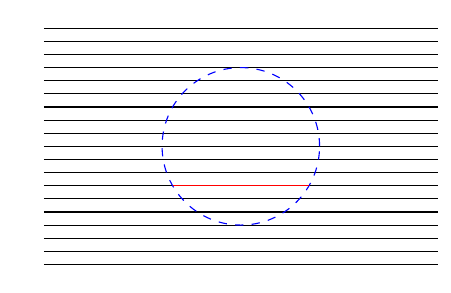
\begin{tikzpicture}[scale=0.5]
  % Draw 10 vertical lines closely bunched together
  \foreach \x in {0,1,2,...,18} {
    \draw (0,\x/3) -- (10,\x/3);
  }
  
  % Draw the circle
  \draw[dashed,blue] (5,3) circle (2);
  
  % Highlight one of the line segments in the circle
  \draw[red] (5-1.73,2) -- (5+1.73,2);
\end{tikzpicture}
\caption{$N'$ is the collection of black lines. The interior of the blue disc is an open subset of the plane $U$, and the red segment is a plaque.}
\end{center}
\end{figure}

Some commentary before we slot this into our hierarchy.
The definition of submanifold in~\cite{Sharpe1997} requires a collection of charts $(U_\alpha, \varphi_\alpha)$ of $M$ covering $\overline{N'}$ such that the connected components of $U_\alpha \cap N'$ are all flat plaques.
This has the effect of excluding the following example.
Consider $N$ as a countable collection of spheres and take $\phi : N \to \bbR^3$ to be the map that embeds the $k$th sphere as $\partial B(k^{-1}, 0.5(k+1)^{-2})$; one has a sequence of non-overlapping spheres decreasing in size with the origin as a limit point.
In particular any neighbourhood $U$ of the origin must contain a sphere as a connected component of $U \cap N' = \phi[N]$, but a sphere cannot be a flat plaque.
Sharpe calls this an `odd limit point', but it seems no more odd than a collection of lines immersed as $\{n^{-1}\} \times \bbR \subset \bbR^2$, which is allowed by the definition.
If one truly wishes to avoid odd limits, an embedded submanifold is the correct notion.
Instead, it would be better to say that Sharpe is concerned with foliations, and this shrinking chain of spheres cannot be part of a regular foliation.
For embedded submanifolds the subspace and submanifold topologies coincide~\cite[Prop~1.2.9]{Sharpe1997}.
The example of the dense wrapping of the line around a torus is the classic example of a submanifold in Sharpe's sense that is not embedded.

It is also important that we use paracompact manifolds,which is equivalent to each connected component being second countable.
This is because a subset of $M$ need not be second countable in the submanifold topology.
Consider the example of the irrational numbers in the real line.
The flat plaques are the sets $\{x\}$ for any irrational $x$.
Thus the submanifold topology is the discrete topology, which is not second-countable.

\begin{theorem}
\label{thm:weakly embedded submanifold}
\textup{\cite[Thm~1.2.7]{Sharpe1997}\cite[Lems~I.2.15--17]{Kolar1993}} \\
Let $N' \subset M$ be a subset.
Suppose for every point $x \in N'$ there is a chart making $C(N'\cap U,x)$ is a flat plaque of dimension $n$.
Let $N$ be the set $N'$ with the submanifold topology and a smooth atlas comprised of the plaque charts.
Then $N$ is a manifold and the inclusion map is a weak embedding.
Conversely, if $\phi : N \to M$ is a weak embedding then this reconstructs the atlas of $N$.
\end{theorem}
\begin{proof}
Because we have weakened the conditions, the proof in~\cite[Thm~1.2.7(i)]{Sharpe1997} no longer works.
I am not completely convinced by~\cite[Lems~I.2.15--17]{Kolar1993} because it uses a Riemannian metric, but the usual proof that a Riemannian metric induces the topology of a space already assumes that you have a topological manifold.
The arguments below attempt to add fill out the details on their idea.

A subspace of a Hausdorff space is Hausdorff, and the submanifold topology is finer than the subspace topology.
Hence $N$ is Hausdorff too.
We can argue in the same way for the other separation axioms, and that $N$ is locally compact.

To show that $N$ is paracompact, we need to show that each connected component $N_0 \subset N$ is second countable.
Necessarily $N_0$ is contained in a connected component $M_0 \subset M$, which is second countable since $M$ is paracompact.
We apply Urysohn's metrization theorem, which says that $M_0$ is metricizable, to get a distance function $d$.
Now $N_0$ is a metric space using the restriction of $d$, but this induces the subspace topology, not necessarily the submanifold topology.
Instead we use the intrinsic distance function $d'$, which is the infimum of path lengths in $N_0$ measured with $d$.

In general, $d' > d$, and we may worry that although $N_0$ is path connected, some of the paths might be infinitely long, and hence $N_0$ would not be a metric space.
To see that this is not the case, for any point $x \in N_0$ consider first a flat plaque $W \ni x$.
We use $\varphi$ to move everything to $\bbR^m$.
Shrinking the chart if necessary, we can assume that $U$ is convex.
$d$ induces a distance function on $\bbR^n \supset W$.
Therefore the intrinsic distance between any points of $W$ is finite, because the length of a chord is an upper bound.
A path between two points of $N_0$ is compact, and therefore covered by finitely many `convex' flat plaques.
The triangle equality now ensures that the path length is finite.

In fact for any open set $V$ of $N_0$, choose any point $x \in V$.
We consider the convex flat plaque centered at $x$ from the previous paragraph.
The set $V \cap W$ is an open subset of the affine subspace, so there is an open set $\tilde{V} \subset U \subset \bbR^n$ with $\tilde{V} \cap W = V \cap W$.
Because $d$ generates the topology of $U$, there is some ball $B_d(x,r) \subset \tilde{V}$.
By a standard argument, any path that leaves $B_d(x,r) \cap W$ has length at least $r$, so $B_{d'}(x,r) \subset B_d(x,r) \cap W$. 
Hence we have found an open ball with respect to $d'$ centered at $x$ contained in $V$.
As we can do this for every point of $V$, $d'$ induces the submanifold topology.

Lastly,~\href{https://math.stackexchange.com/questions/10885/non-separable-locally-compact-connected-metric-space}{MSE} tells us that a connected locally-compact metric space is second countable.
By definition, the plaque charts form a smooth atlas.
Therefore we have shown that $N_0$ is a manifold.

That this is a weak embedding is~\cite[Thm~1.2.7(iii)]{Kolar1993}.

The converse follows from~\cite[I.2.15~Lemma]{Kolar1993} (the construction can be carried out on the image of a weak embedding) and~\cite[Lemma~1.1.41]{Sharpe1997} (a weak embedding is compatible with a unique manifold structure).
\end{proof}

Finally, by \cite[Thm~1.2.11]{Sharpe1997} proper submanifolds are automatically embedded, so we have a strict hierarchy of conditions.
The standard example of an embedded submanifold that is not proper is $(0,1) \subset \bbR$.
We see that a sequence in $N$ may converge to a point of $M\setminus N$.

These constructions answer the question of how to endow a subset with a manifold structure.
There is the possibility however that there are different constructions.
Warner addresses these concerns with the following theorem: 
\begin{theorem}
\label{thm:submanifolds}
\textup{\cite[Remark~1.33]{Warner1983}}
\begin{enumerate}
\item Let $M$ be a manifold and $A$ a subset of $M$. Fix a topology on $A$. Then there is at most one manifold structure on $A$ such that $(A,\phi)$ is an immersed submanifold of $M$, where $\phi$ is the inclusion map.
\item Again let $A$ be a subset of $M$. If $A$ with the subspace topology has a manifold structure such that $(A,\phi)$ is an immersed submanifold of $M$, then it is the unique topology on $A$ such that there exits a manifold structure for which $(A,\phi)$ is an immersed submanifold of $M$.
\end{enumerate}
\end{theorem}

We generalise Part (b) slightly below.
This generalisation is stronger than~\cite[Lem~2.1.41]{Sharpe1997}, because we only require the inclusions to be injective immersions, not weak embeddings.

\begin{theorem}
\label{thm:unique manifold structure}
Let $A$ be a subset of $M$. 
If $A$ with the submanifold topology has a manifold structure such that $(A,\phi)$ is an immersed submanifold of $M$, then it is the unique topology on $A$ such that there exits a manifold structure for which $(A,\phi)$ is an immersed submanifold of $M$.
\end{theorem}
\begin{proof}
First we address the relationship between the manifold structure on $A$ and the plaque charts.
For any function $A \hookrightarrow M$ that is an immersion at $p$ the constant rank theorem gives us a plaque chart of $A$ at $p$.
Applying this to the inclusion $\phi$ and at every point we get that $A$ is a weakly embedded submanifold.
By Part (a) of the previous theorem this is the unique manifold structure on $A$ with the submanifold topology (the manifold structure supposed in this theorem and the plaque charts belong to the same maximal atlas).

Now we move on to the statement in the theorem.
For clarity, let $B$ the manifold that has the same points as $A$ but a different topology and manifold structure, and let its inclusion be $\psi : B \hookrightarrow M$.
In terms of points, the composition $\phi^{-1} \circ \psi : B \to A$ is the identity map, so bijective.
We know that $(A,\phi)$ is a weak embedding.
Hence $\phi^{-1} \circ \psi$ is in fact a smooth map of manifolds.
It must also be an immersion: if there is a smooth path $\alpha$ in $B$ such that $\phi^{-1} \circ \psi \circ \alpha$ represents the zero vector then $\psi \circ \alpha$ represents the zero vector in $M$ by applying $\phi$ and so $\alpha$ represents the zero vector using that $\psi$ is an immersion. 
At the final step of the proof of Part (b) of the above theorem, Warner uses his Exercise~1.6 to conclude that a smooth bijective immersion is a diffeomorphism.
We do the same.
\end{proof}


\subsection{Lie Brackets and Distributions}

It is common in a course on manifolds to study vector fields and their integral curves.
The key local result is
\begin{theorem}[Picard-Lindelöff]
\textup{\cite[Theorem~2.1.1]{Sharpe1997}}\cite[Theorem~1.2.1]{Ivey} \\
Let $F : J \times U \subset \bbR\times\bbR^n \to \bbR^n$ be a smooth time-dependent vector field. 
Assume $0 \in J$. 
Consider $u : \bbR \to U$ the system of ODEs $u'(t) = F(t,u(t))$.
For any $c \in U$ there exists a $\varepsilon > 0$ such that there is a unique solution smooth solution on $(-\varepsilon,\varepsilon)$ with $u(0) = c$.
Moreover, for any $p \in U$ there is an open neighbourhood $p \in V \subset U$, $\varepsilon > 0$ and smooth map $u : (-\varepsilon,\varepsilon) \times V \to U$ such that $u(\cdot,c)$ is the unique solution with initial condition $c$.
\end{theorem}

If one has a smooth vector field on a manifold, then we can ask for a curve $\gamma$ through $p = \gamma(0)$, called an integral curve, such that the tangent vectors of $\gamma$ are equal to the vector field.
In other words, the integral curve is a solution to the time-independent ODE $\gamma'(t) = X(\gamma(t))$.
this theorem provides for the existence of integral curves of the vector field in every coordinate chart, and uniqueness means that they can be patched together to give unique maximal integral curves through every point.

The set of integral curves of a vector field $X$ define a flow of the manifold: $\tilde{X}_t(p)$ is defined to be equal to the integral curve of $X$ through $p$ at time $t$ (ie $t \mapsto \tilde{X}_t(p)$ is the integral curve).
This is a smooth function defined on a subset of $\bbR \times M$ (treating the subscript as the first variable here), in particular containing some neighbourhood $(-\varepsilon,\varepsilon) \times U$ of any point $(0,p)$.
Uniqueness of the integral curves means that this flow is reversible.
Moreover, if the vector field is nonzero at a point, there is a chart containing that point where the vector field is the first coordinate vector $\partial_1$ and the flow is translation.
In the other direction, the derivative of the flow with respect to $t$ at $t=0$ gives back the vector field $X$.

The flow provides a way to connect points of a manifold with neighbouring points, and so can be used to define a derivative, called the Lie derivative.
For example, for a function $f$
\[
\mathcal{L}_X f
= \lim_{h \to 0} h^{-1} \left( f \circ \tilde{X}_h - f \right)
= \left.\frac{d}{dt}\right|_{t=0} f \circ \tilde{X}_t
\]
is, by the chain rule, equal to $\langle X, f\rangle$.
The Lie derivative of a vector field is likewise defined by
\[
\mathcal{L}_X Y
= \lim_{h \to 0} h^{-1} \left( d\tilde{X}_{-h}(Y \circ \tilde{X}_h) - Y \right)
= \left.\frac{d}{dt}\right|_{t=0} d\tilde{X}_{-t} \circ Y \circ \tilde{X}_t
\]
which is well-defined since $d\tilde{X}_{-h}$ takes $T_{\tilde{X}_h(p)}M$ to $T_pM$.
Most importantly, the Lie derivative of a vector field is a type of commutator.
This is easiest to calculate in local coordinates, specifically the ones adapted to the flow of $X$~\cite[Thm~9.38]{Lee2012}.
If $Y(p) = Y^i(p) \partial_i|_p$ then
\begin{align*}
d\tilde{X}_{-h}(Y \circ \tilde{X}_h) (p)
&= d\tilde{X}_{-h} \left( Y^i(p + (h,0,\ldots)) \partial_i|_{\tilde{X}_h(p)} \right)
= Y^i(p + (h,0,\ldots)) \partial_i|_{p} \\
\mathcal{L}_X Y (p)
&= \lim_{h \to 0} h^{-1} \left( Y^i(p + (h,0,\ldots)) - Y^i(p) \right) \partial_i|_{p}
= \frac{\partial Y^i}{\partial x_1} \partial_i|_{p}.
\end{align*}
On the other hand, this is the commutator of $X$ and $Y$
\begin{align*}
[X,Y]
= \frac{\partial Y^i}{\partial x_1} \partial_i - Y^i\frac{\partial 1}{\partial x_i} \partial_1
= \frac{\partial Y^i}{\partial x_1} \partial_i.
\end{align*}
One can check that the commutator of two vector fields is a well-defined vector field, independent of the coordinates.
Therefore $\mathcal{L}_X Y = [X,Y]$.

From this commutator formula, most of the properties of the Lie derivative of vector fields easily follow.
For us, the most important are anti-symmetry $[X,Y] = -[Y,X]$ and the Jacobi identity $[X,[Y,Z]] = [[X,Y],Z] + [Y, [X,Z]]$.
There is also a generalisation of adapted coordinates to sets of linearly-independent commuting vector fields: around each point there is a chart whose coordinates vector fields are the given vector fields.

We will need a generalisation that deals with vector fields that are not commuting.
To motivate why this is geometrically interesting and not just generalisation for its own sake, consider a submanifold $N$ inside $M$.
At each point $p \in N$ we can consider the vector subspace $T_pN \subset T_pM$.
At least locally, we can describe these subspaces as the span of independent vector fields.
The natural question is the converse: given a set of independent vector fields on $M$, does there exist a submanifold $N$ whose tangent space is their span?
For a single vector field, the answer is affirmative, namely the integral curve.

\begin{definition}
\textup{\cite[2.2.1,.2.2.2,2.3.2]{Sharpe1997}} \\
An $r$-dimensional distribution $\mathcal{D}$ on $M$ is a choice of an $r$-dimensional subspace $\mathcal{D}_p$ of $T_p M$ at every point $p \in M$.
It is called smooth if every point has a neighbourhood and smooth vector fields $\{X_1, \dots, X_r \}$ that span the subspaces.
This is called a local basis for $\mathcal{D}$.
Equivalently, an $r$-dimensional distribution is an rank $r$ subbundle of $TM$.

A set of vector fields is called algebraically involutive if their Lie brackets are contained in their span.
Given two sets of vector fields with the same span, one is algebraically involutive if and only if the other is.
Therefore algebraically involutive is a property that is defined for distributions.

A distribution is called integrable if every point has a coordinate neighbourhood in which the distribution is spanned by coordinate vector fields.
\\
A connected $r$-dimensional immersed submanifold $N$ is called an integral submanifold of $\mathcal{D}$ if at every point $T_pN = \mathcal{D}_p$.
\end{definition}

Consider the example of nested spheres centered at the origin in $\bbR^3\setminus\{0\}$. 
Their tangent planes define a $2$-distribution.
In a neighbourhood of any point, suitable polar coordinates show that it is smooth and integrable.
However there are not global vector fields spanning this distribution, due to the hairy ball theorem (every vector field on a sphere vanishes at least once).
By definition, any of the spheres is an integral manifold of this distribution.

The important example of a non-integrable distribution is given in $\bbR^3$ by the planes normal to the vector field $n(x,y,z)=(y,-x,1)$~\cite[Ex~2.3.1]{Sharpe1997}.
There can be no integral manifold containing the origin.
Suppose there were.
Because the tangent plane at the origin is the $xy$-plane, we know that there is a neighbourhood where is a graph over $x$ and $y$.
Now take a small loop in the integral manifold around the origin lying in this neighbourhood.
It's height is monotonic, it doesn't close up.
This is a contradiction.
A local basis at the origin is given by $X_1 = \partial_x - y \partial_z$, $X_2 = \partial_y + x\partial z$.
Observe that $[X_1,X_2] = 2\partial_z$, so that it is not algebraically involutive.


If a distribution is integrable, then every point has an integral submanifold through it, just by taking a coordinate plane in an appropriate chart.
And if there is an integral submanifold of the distribution at a point, the local basis of the distribution gives a vector field on it.
So then the Lie bracket is again tangent to the integral submanifold, showing that the vector fields are algebraically involutive at that point.
Hence algebraic involutive is a necessary condition to the existence of an integral submanifold.

\begin{theorem}[Frobenius' theorem]
\textup{\cite[Thm~2.4.1,~Cor~2.4.2]{Sharpe1997}\cite[Thm~1.60,~1.62]{Warner1983}\cite[Thm~19.2]{Lee2012}} \\
A distribution is integrable if and only if it is algebraically involutive.
An integral submanifold is weakly embedded.
\end{theorem}
\begin{proof}
It suffices to show that locally every distribution can be spanned by linearly-independent commuting vector fields.
If it can be, then by the discussion above there is an adapted coordinate system, and the connected component of the integral submanifold in this chart through a given point is a coordinate plane, thus a flat plaque.

Since this is a local question, we will work in a local coordinate.
Let $\mathcal{D}$ be rank $r$ and take any local basis $X_1, \dots, X_r$.
By rotating coordinates, assume that at $p$ the basis is complementary to $\partial_{r+1},\dots,\partial_{m}$.
Let $\pi$ be the projection onto the first $r$ coordinates.
$d\pi|_D : D \to TU$ is a smooth bundle homomorphism, and it is an isomorphism at $p$ by our set-up.
Hence there is a neighborhood of $p$ where it is invertible.
Hence $Y_i = (d\pi|_D)^{-1} \partial_i$ is also a local basis of $\mathcal{D}$ at $p$.
But by the naturality of the Lie bracket 
\[
[Y_i, Y_j] 
= [(d\pi|_D)^{-1} \partial_i, (d\pi|_D)^{-1} \partial_j]
= (d\pi|_D)^{-1} [\partial_i, \partial_j]
= 0.
\qedhere
\]
\end{proof}

We can use uniqueness to unite integral submanifolds of a distribution into their maximal connected components.
Each of these is called a leaf and the collection of leaves is a foliation.

Perhaps let us revisit the example from the previous section of a weakly embedded submanifold that is not a submanifold in the sense of Sharpe, the shrinking spheres.
There is no distribution on $\bbR^3$ with this as an integral submanifold. 
If we take a sequence of corresponding points on the spheres, $p_n = c_n + r_n \omega$ for $\omega \in \bbS^2$ for $c_n,r_n$ the centers and radii of the spheres, the limit is the origin. 
But all the tangent planes $T_{p_n}(\partial B(c_n,r_n))$ are parallel, so their limit is just any of them translated to the origin.
Taking several such sequences, we see that the distribution cannot be continuous at the origin.


% There is also a formulation of Frobenius' theorem in terms of differential forms.
% We can define the annihilator of a distribution as the algebraic ideal generated by the one-forms such that $\omega(v) = 0$ for all $v \in \mathcal{D}_p$.
% By this we mean all $C^\infty$-linear combinations and wedge products.
% Conversely, the kernel of an algebraic ideal of differential forms generated locally by $m-r$ independent one-forms is a distribution.
% The theorem then says that $\mathcal{D}$ is integrable if and only if the ideal contains all its exterior derivatives (it is a differential ideal).
% The proof comes down to the simple formula
% \[
% d\omega(X,Y) = X(\omega(Y)) - Y(\omega(X)) - \omega([X,Y]).
% \]

\subsection{Eigenvalues and Weights}

Eigenvalues and eigenvectors are ubiquitous in linear algebra.
If we are working over $\bbC$, then every linear endomorphism (linear map from a vector space $V$ to itself) has an eigenvalue (root of the characteristic polynomial) and every eigenvalue has an eigenvector $Av_\lambda = \lambda v_\lambda$.
If we can find a basis of eigenvectors, then with respect to this basis the linear operator is a diagonal matrix.
In general however, there may be fewer eigenvectors than the dimension of the vector space.
A standard result in linear algebra says that every matrix is conjugate to a matrix in Jordan normal form, unique up to reordering of the blocks.

Going further, we may ask what can be said of two linear endomorphisms $A,B$.
The key observation is to consider commuting operators.
If $A$ and $B$ commute then $B$ preserves the eigenspaces  eigenspaces of $A$:
\[
(A- \lambda I) (Bv) 
= B(A- \lambda I) v
= 0.
\]
Therefore $B$ restricts to an endomorphism on each of the eigenspaces of $A$.
Imposing different conditions on $A$ restricts the possible decompositions of $B$.
For example, if $A$ is diagonalizable (so $V$ decomposes as the direct sum of the eigenspaces of $A$) then on each eigenspace of $A$ we can choose a basis that puts $B$ into Jordan normal form.
Hence $A$ and $B$ can simultaneously conjugated to normal form.
Or if $A$ is diagonalizable and has no repeated eigenvalues, ie its eigenspaces are one dimensional, then these must also be eigenspaces of $B$.
Hence $A$ and $B$ are simultaneously diagonalizable.

This argument can be applied inductively to a finite set $\{A_1,\dots,A_k\}$ of pairwise commuting endomorphisms.
It also extends to a commuting family of operators $\mathcal{A} = \vspan\{A_1,\dots,A_k\}$, a linear subspace of $\End(V)$ such that all operators are pairwise commuting.
These are effectively equivalent, since a family is pairwise commuting if and only if a basis is pairwise commuting.
Likewise, $v$ is a simultaneous eigenvector for $\{A_1,\dots,A_k\}$ if and only if it is a simultaneous eigenvector for every operator of $\mathcal{A}$.
The eigenvalues are not completely independent:
\[
\lambda v
= Av 
= (a_1A_1 + \dots + a_kA_k)v
= a_1 \lambda_1 v + \dots + a_k \lambda_k v
= (a_1 \lambda_1 + \dots + a_k \lambda_k )v.
\]
We understand the eigenvalue of $v$ to be a linear function 
\[
\lambda : \mathcal{A} \to \mathbb{K}, 
\quad
\lambda(A) = a_1 \lambda_1 + \dots + a_k \lambda_k .
\]
Understood in this way, it is more common to call $\lambda$ a \emph{weight} of the commuting family $\mathcal{A}$, $v$ a \emph{weight vector}, and the set of vectors $v$ with $Av = \lambda(A)v$ the \emph{weight} space~\cite[Definition~A.14]{Hall2015}.

As an aside, the descriptor ``weight'' should probably replace ``eigen-'' even in the single operator case.
Consider an operator $A$ with a $2$-weight vector $v$ and a $3$-weight vector $w$.
Then of course $A(v+w) = 2v + 3w$, which is a weighted sum.

We finish with an example.
Let $\mathcal{A}$ be the set of diagonal $n\times n$ matrices.
Then a basis for this family is $A_i = e_{ii}$, with $1$ at the $i$th position on the diagonal.
$e_i$ is a $1$-weight vector of $A_i$ while all vectors of $\vspan\{e_1,\dots,\hat{e}_i,\dots,e_n\}$ are $0$-weight (in the kernel).
These are all diagonal (in particular simultaneously diagonal) so there should be a basis of weight vectors.
Indeed, this is just the standard basis $\{e_1,\dots,e_n\}$.
The weight of $e_i$ is the linear form
\[
A = \operatorname{diag}(a_1,\dots,a_n) \mapsto a_i
\]
because $A e_i = a_i$.


% !TEX root = lie-groups.tex
\section{Lie Groups}

Historically and in practice, Lie groups arise first as the study of the transformation of geometric objects.
Let us consider the example of a sphere in euclidean space.
There are in a sense three ways to rotate a sphere.
Choose a point on the equator of a sphere.
You can rotate the sphere so that this point moves towards a pole (y-axis rotation), so that this point moves along the equator (z-axis rotation), or so that the point is stationary (x-axis rotation).
Moreover these rotations are continuous in a way that rotating an equilateral triangle is not, because at each stage of rotation the sphere as a whole occupies the same space.

How should we describe the rotations of a sphere?
First observe that antipodal points remain antipodal, so the rotation of a sphere extends to a linear transformation of $\bbR^3$.
Hence any rotation $R$ can be described by a real $3\times 3$-matrix.
Moreover rotation is length and angle preserving, so $\langle Rx, Ry \rangle = \langle x, y \rangle$.
This holds exactly if $R^TR = I$, which gives us the orthogonal group
\[
\lgO(3) = \{ R \in \Mat(3,\bbR) \mid R^TR = I \}.
\]
We can understand the defining equation as saying that the columns of $R$ are an orthonormal basis of $\bbR^3$.
Indeed they are the images of the standard basis of $\bbR^3$ under $R$.
By rotations we mean proper rotations, which are by definition orientation preserving, so we want that the columns of $R$ are a right handed basis.
That leads to the special orthogonal group
\[
\lgSO(3) = \{ R \in \lgO(3) \mid \det R = 1 \}.
\]
The group operation is composition of operators, ie matrix multiplication.
Both groups clearly contain the identity $I$.
The property $R^T R = I$ implies $(\det R)^2 = 1$, so these are invertible matrices.
Therefore they really are groups.
Moreover the sign of the determinant can be used to distinguish a proper rotation from an improper one.
% The later group are the (proper) rotations, the former is a group that includes reflections.

Heuristically, we have nine choices for the matrix of $R$ subject to the restriction each of the three columns must be unit length and the restriction that pairs of columns must be orthogonal (six restrictions total).
This agrees with the three degrees of freedom we argued for above.
To see this is a manifold however we consider a function $f$ from $\Mat(3,\bbR)$ to the symmetric matrices given by $f(R) = R^TR$.
The orthogonal matrices are exactly $\lgO(3) = f^{-1}(I)$.
The derivative at $R$ in the direction $S$ is $f'(R)(S) = R^TS + S^T R = R^T S + (R^T S)^T$.
At a point $R \in \lgO(3)$ this is surjective in $S$: for any symmetric matrix $Y$ let $S = \frac{1}{2}RY$.
Hence $f$ is full rank at every point $R \in \lgO(3)$ and by the implicit function theorem $\lgO(3)$ is an embedded submanifold of $\Mat(3,\bbR) \cong \bbR^9$.
The symmetric matrices are dimension $6$, so in fact our heuristic has been formalised to a rigorous argument.

The group operation, matrix multiplication, is a smooth operation on the set of matrices because it is polynomial.
Therefore it is also smooth when restricted to an embedded submanifold.
Similarly inversion is an everywhere defined rational function on the open set of invertible matrices, so also smooth on $\lgO(3)$.
This makes $\lgO(3)$ and $\lgSO(3)$ Lie groups.

Now that we know that $\lgO(3)$ is a manifold, we can ask about its connected components.
Intuitively we can rotate any right handed frame $R \in \lgSO(3)$ to the standard basis $I$, so $\lgSO(3)$ is connected.
Because it contains the identity, it is called the identity component.
On the other hand, the reflection in the plane $x_1 = 0$ has determinant $-1$ whereas $\det I = 1$.
Determinant is continuous (polynomial) function on matrices and as already noted $R \in \lgO(3)$ implies $\det R = \pm 1$, so this reflection is not in the identity component.
Composing an improper rotation with this reflection gives a proper rotation and vice-versa. Therefore the subset of $\lgO(3)$ with $\det R = -1$ is also a connected component of $\lgO(3)$.
In conclusion, $\lgSO(3)$ is connected and $\lgO(3)$ has two diffeomorphic components.

To understand the topology of $\lgSO(3)$ an alternate description is useful.
Every rotation of $\bbR^3$ is rotation around an axis.
More precisely, we can describe the rotation axis by a unit vector $u$ such that the rotation is right handed by an angle $\theta$ in the range $[0,\pi]$.
Thus the rotations can be described by the closed unit ball $\theta u \in \overline{B(0,1)}$.
The origin is rotation by angle $0$ with the axis of rotation irrelevant.
But similarly, rotation by $\pi$ around $u$ and $-u$ are the same rotation.
Thus $\lgSO(3)$ can be modelled as the closed unit ball with antipodal points on the boundary identified, the real projective space $\RP^3$.

In this model it is easy to understand the fundamental group.
Take any closed loop in $\lgSO(3)$.
If it lies entirely in $B(0,1)$ then it can be contracted to a point.
% If it meets $\partial B(0,1)$ in one point then we may describe it as a path $\gamma : (0,1) \to B(0,1)$ with $\gamma(1) = - \gamma(0) \in \partial B(0,1)$. 
Otherwise it can be divided into a collection of segments $\gamma_i : (0,1) \to B(0,1)$ with $\gamma_{i+1}(0) = \pm \gamma_i(1) \in \partial B(0,1)$ and $\gamma_1(0) = \pm \gamma_n(1) \in \partial B(0,1)$.
These conditions ensure that the segments connect up to a loop in $\RP^3$.
We call the number of negative signs the index of the loop.
If $\gamma_{i+1}(0) = \gamma_i(1)$ then it is possible to move this point into the interior of $B(0,1)$ and fuse these two segments together into a single segment.
This doesn't change the index of the loop.
As an extreme case, if the index is zero, then we can move all the endpoints of the segments off $\partial B(0,1)$ and contract the loop to a point.
So without loss of generality, assume that all the signs are negatives.
\begin{center}
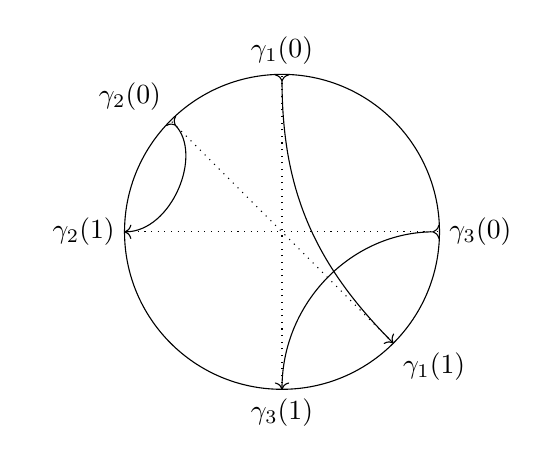
\begin{tikzpicture}
    % Circle
    \draw (0,0) circle (2cm);
    
    % Curve 1
    \draw[>->] (90:2cm) to[out=270, in=135] (-45:2cm);
    \node at (90:2cm) [above] {$\gamma_1(0)$};
    \node at (-45:2cm) [below right] {$\gamma_1(1)$};

    \draw[dotted] (-45:2cm) -- (135:2cm);
    
    % Curve 2
    \draw[>->] (135:2cm) to[out=-45, in=0] (180:2cm);
    \node at (135:2cm) [above left] {$\gamma_2(0)$};
    \node at (180:2cm) [left] {$\gamma_2(1)$};

    \draw[dotted] (180:2cm) -- (0:2cm);

    % Curve 3
    \draw[>->] (0:2cm) to[out=180, in=90] (-90:2cm);
    \node at (0:2cm) [right] {$\gamma_3(0)$};
    \node at (-90:2cm) [below] {$\gamma_3(1)$};

    \draw[dotted] (-90:2cm) -- (90:2cm);
\end{tikzpicture}
\begin{tikzpicture}
    % Circle
    \draw (0,0) circle (2cm);
    
    % Curve 1
    \draw[>->] (90:2cm) to[out=270, in=110] (0:2cm);
    \node at (90:2cm) [above] {$\gamma_1(0)$};
    % \node at (-45:2cm) [below right] {$\gamma_1(1)$};

    % \draw[dotted] (-45:2cm) -- (135:2cm);
    
    % Curve 2
    \draw[>->] (180:2cm) to[out=45, in=180] (150:1.5cm) to[out=0, in=0]  (180:2cm);
    % \node at (135:2cm) [above left] {$\gamma_2(0)$};
    \node at (180:2cm) [left] {$\gamma_2(0) = \gamma_2(1)$};

    \draw[dotted] (180:2cm) -- (0:2cm);

    % Curve 3
    \draw[>->] (0:2cm) to[out=180, in=90] (-90:2cm);
    \node at (0:2cm) [right] {$\gamma_1(1)=\gamma_3(0)$};
    \node at (-90:2cm) [below] {$\gamma_3(1)$};

    \draw[dotted] (-90:2cm) -- (90:2cm);
\end{tikzpicture}
\end{center}
If there is more than one segment, we can move $\gamma_1$ and $\gamma_2$ such that $\gamma_1(0)$ and $\gamma_2(1)$ remain fixed (so no other segments are affected) but $\gamma_2(0)$ is moved to $\gamma_2(1)$ (so necessarily $\gamma_1(1) \to - \gamma_2(1)$).
Then $\gamma_2$ can be contracted to the constant map $\gamma_1(1) = -\gamma_2(0) = -\gamma_2(1) = \gamma_3(0)$.
This means that we can eliminate $\gamma_2$ and fuse $\gamma_1$ and $\gamma_3$ into a single segment.
In particular, the index has decreased by two.
The act of moving part of an arc from one part of the boundary to the opposite side increases the index by two.
Hence the parity of the index is a homotopy invariant.
This has proven that the fundamental group of $\RP^3$, and hence $\lgSO(3)$, is $\bbZ_2$:
any loop with an even number of segments can be contracted to a point, whereas any loop with an odd number of segments can be reduced to a diameter.


\subsection{Basic Notions}

\begin{definition}
\label{def:lie group}
\textup{\cite[3.1]{Warner1983}\cite[Definition~1.20]{Hall2015}} \\
A \emph{Lie Group} is a $G$ manifold with a group structure such that multiplication $\mu : (g,h) \mapsto gh$ and inversion $\iota : g \mapsto g^{-1}$ are smooth.
\end{definition}

Many familiar manifolds are also Lie groups in natural ways.
For example, the reals $\bbR$ under addition, the multiplicative group of the complex numbers $\bbC^\times$, and the circle $\bbS^1 = \{ z \in \bbC^\times \mid |z| = 1 \}$.
The product of two Lie groups is a Lie group, using the product manifold and product group structures.
This gives us euclidean space $\bbR^n$ with vector addition and the torus $\bbT^n = (\bbS^1)^n$ as further examples.

Many definitions carry over naturally by requiring both a manifold-theory and a group-theory property.
For example
\begin{definition}
\textup{\cite[3.13]{Warner1983}} \\
A \emph{homomorphism of Lie groups} is a smooth map $\phi : G \to H$ that is also group homomorphism.
If $\phi$ is further a diffeomorphism, then we say it is an \emph{isomorphism of Lie groups}.
\end{definition}


Given any Lie group $G$, we can construct the opposite group $G^{op}$.
As a set and a manifold they are the same, but multiplication is given by $\mu^{op}(g,h) = \mu(h,g)$.
Observe that inversion is an isomorphism of Lie groups between $G$ and $G^{op}$.
By the definition of a Lie group, $\iota$ is a diffeomorphism.
It is also a homomorphism of the group structure since
\[
\mu^{op}(\iota(g),\iota(h))
= \mu(\iota(h),\iota(g))
= h^{-1}g^{-1}
= (gh)^{-1}
= \iota(\mu(g,h)).
\]

It is often fruitful to fix an element of the group and look at its action.
We have the left action $L_g = \mu(g,\cdot) : G \to G$ and the right action $R_g = \mu(\cdot,g)$.
It is customary to primarily work with the left action.
There is no loss of generality in doing so, because the right action in $G$ is the left action in $G^{op}$.

Sometimes however a different concept is more appropriate for Lie theory.
In manifold theory one is mostly concerned with embedded submanifolds, while in Lie theory immersed submanifolds are more useful:
\begin{definition}\label{Def:subgroup}
\textup{\cite[3.17]{Warner1983}, contrast~\cite[\S{}7.1]{Fulton2004}}\\
A \emph{Lie subgroup} $(H,\varphi)$ of a Lie group $G$ is a Lie group $H$ and an injective immersion $\varphi : H \to G$ that is also a homomorphism.
It is called a \emph{closed Lie subgroup} if $\varphi(H)$ is further closed.
\end{definition}

In fact later we will improve the regularity by showing that all Lie subgroups are weakly embedded and that a Lie subgroup is embedded if and only if it is closed.






\subsection{Examples}

There are many interesting properties that Lie groups can possess, and we give a quick tour of them with examples.

All finite groups are also Lie groups using the discrete topology to make them $0$-dimensional manifolds.
These are not central examples of Lie groups, whose essential character is their `continuity', but they are useful to describe non-connected Lie groups.
For example, we have seen that the $\lgSO(3)$ is the component of $\lgO(3)$ that contains the identity.
In fact $\lgO(3)$ is the product of $\lgSO(3)$ and $C_2$ the group with two elements.
Generalising, the identity component $G_0$ of a Lie group $G$ is a Lie group.
To prove this, note that $\mu(I,I) = I$ and $\iota(I) = I$, so the images of $G_0\times G_0$ under multiplication and $G_0$ under inversion, which are connected, are both contained in $G_0$.
If $g$ belongs to another connected component $G_1$ then multiplication with $g$ is a diffeomorphism between $G_0$ and $G_1$.
In this way, every Lie group with finitely many connected components is the product of its identity component and a finite group.
For this reason we usually consider connected Lie groups of positive dimension.

As in group theory, we have abelian and non-abelian groups.
Abelian Lie groups include $\bbR^n$ and $\bbT^n$ and $\lgO(3)$ and $\lgSO(3)$ are examples of non-abelian groups.
As we will see later, the abelian Lie groups are easy to classify.

Perhaps the most important category of Lie group are the matrix Lie groups~\cite[Definition~1.4]{Hall2015}.
First we have the general linear group $\lgGL(n,\bbC)$, the set of $n\times n$ invertible matrices with complex entries.
This can be considered as an open subset of $\bbC^{n^2}$, so it is a manifold. And just as for $\lgO(3)$ the group operation is polynomial and group inversion is rational without zeroes of the denominator, hence both are smooth.
A matrix group is any closed Lie subgroup of $\lgGL(n,\bbC)$.
As a special case we have the real matrix groups, which are subsets of the (real) matrix group $\lgGL(n,\bbR)$.

We have already seen the real matrix groups $\lgO(3)$ and $\lgSO(3)$.
As the notation suggests, these belong to families indexed by the size of the matrices.
We have the following families of matrix groups
\begin{align*}
\lgSL(n,\bbC) &= \{ A \in \lgGL(n,\bbC) \mid \det A = 1 \} \\
\lgSL(n,\bbR) &= \{ A \in \lgGL(n,\bbR) \mid \det A = 1 \} \\
\lgU(n) &= \{ A \in \lgGL(n,\bbC) \mid \bar{A}^T A = I \} \\
\lgSU(n) &= \{ A \in \lgU(n) \mid \det A = 1 \} \\
\lgO(n) &= \{ A \in \lgGL(n,\bbR) \mid A^T A = I \} \\
\lgSO(n) &= \{ A \in \lgO(n) \mid \det A = 1 \}.
\end{align*}
If we give $\bbC^n$ the standard inner product $\langle v,w \rangle = \bar{v}^Tw$ then unitary matrices are exactly the linear transformations that preserve it.
In this way the orthogonal groups are the real counterparts to the unitary groups.
The following trick shows that $\lgU(n)$ is compact: As a vector in $\bbC^{n^2}$ the square of the norm of $A \in \lgU(n)$ is $\tr(\bar{A}^T A) = \tr I = n$, thus $\lgU(n)$ is bounded.
Thus all closed subsets, such as $\lgSU(n), \lgO(n),\lgSO(n)$, are also compact.

There are also the symplectic groups.
Like $\lgU$ and $\lgO$ they preserve a bilinear form.
Let 
\[
\Omega = \begin{pmatrix}
0 & I_n \\ - I_n & 0
\end{pmatrix}
\]
be a $2n\times 2n$ matrix in block form and define
\begin{align*}
\lgSp(2n,\bbC) &= \{ A \in \lgGL(2n,\bbC) \mid A^T\Omega A = \Omega \} \\
\lgSp(2n,\bbR) &= \{ A \in \lgGL(2n,\bbR) \mid A^T\Omega A = \Omega \} \\
\lgSp(n) &= \lgSp(2n,\bbC) \cap \lgU(2n).
\end{align*}
The notation around $\lgSp(n)$ is a bit confusing, but the point is to make a compact group.
Indeed $\lgSp(n)$ is called the compact symplectic group.
Together, these examples are called the classical groups and they will figure prominently in the classification of Lie groups.

In Definition~\ref{def:lie group}, a Lie group is a real manifold.
But some of the examples above are in fact complex manifolds: they admit an atlas whose charts map to subsets of $\bbC^n$ and whose transition functions are holomorphic.
Naturally these are called \emph{complex Lie groups}.
$\lgSL(n,\bbC)$ is a complex Lie group because $\det A$ is polynomial in the entries of $A$ and so holomorphic.
The holomorphic version of the implicit function theorem then tells us that it is a complex manifold.
On the other hand $\lgU(n)$ is a complex manifold even though it is a set of complex-valued matrices.


There are of course many other matrix Lie groups.
One could consider groups of matrices preserving other bilinear forms. 
For a concrete example, the subset of diagonal matrices of any of the classical groups is again a matrix group.
In $\lgU(n)$ the diagonal subgroup is $\{\operatorname{diag}(\lambda_1,\dots,\lambda_n)\}$ with $|\lambda_i| = 1$.
We see that this is isomorphic to $\bbT^n$.
The standard terminology is that a Lie group that is isomorphic to a matrix group is called a linear group.
In other words, $\bbT^n$ which is defined as the product of circles, is a linear group but not a matrix group.
Similarly $\bbR$ is a linear group because we can consider real matrices of the form
\[
\begin{pmatrix}
1 & a \\
0 & 1
\end{pmatrix}.
\]
The result of multiplying two such matrices is to add the off-diagonal term.

A similar direction that we will not explore is linear algebraic groups.
These are matrix groups that are algebraic varieties, in particular their defining equations are polynomial.
All the matrix groups above are examples.
Because they are defined by polynomials linear algebraic groups can be defined over any field, not just $\bbC$ and $\bbR$.
However exploring other fields would take us away from the differential geometry point of view that is our focus.
Indeed, many books downplay the differential geometric aspects of Lie theory because they have an eye on this algebraic extension.






\subsection{Subgroups}
First, we remind ourselves of definition \ref{Def:subgroup} to see what a Lie subgroup is. 
First we start with a Proposition that is used quite often:
\begin{Prop}
\textup{\cite[3.18]{Warner1983}}\\
Let $G$ be a connected Lie group, and let $U$ be a neighborhood of the identity $e$. Then 
\begin{align*}
G= \bigcup_{n=1}^{\infty} U^n
\end{align*}
where $U^n$ consists of all $n$-fold products of elements of $U$.
\end{Prop}

\begin{proof}
We will outline the idea of the proof. We consider an open subset $V \subset U$ s.t. $V=V^{-1}$, for example choosing $V = U\cap U^{-1}$. Then we define 
\begin{align*}
H = \bigcup_{n=1}^{\infty} V^n \subset \bigcup_{n=1}^{\infty} U^n.
\end{align*}
By choice of $V$, $H$ satisfies the subgroup condition. Further $H$ is an open subset of $G$ as a union of open sets. In fact for any $g \in G$ the coset $gH$ is open in $G$, since it preimage of $H$ under $(g^{-1} \cdot) : G \to G$.
Now we want to prove that $H$ is also closed. But the complement of $H$ can be written
\[
G \setminus H = \bigcup_{g \in G \setminus H} gH,
\]
a union of open sets.
\end{proof}


For general manifolds there are immersed submanifolds that are not weakly embedded. 
The following theorem rules this out for Lie subgroups; though they are defined only as injective immersion they are in fact stronger.
It also clearly has echos of Theorem~\ref{thm:submanifolds}.

\begin{theorem}
\textup{\cite[3.20]{Warner1983}}\\
If a (abstract) subgroup $A$ of a Lie group $G$ has a manifold structure which makes the inclusion map $\phi: A \to G$ an immersion (and by definition it is injective), then it has a unique manifold structure, and in this manifold structure $A$ is a Lie group and $\phi$ is a weak embedding.
\end{theorem}

\begin{proof}[Sketch of Proof]
We define $\mathcal{D}$ to be the distribution on $G$ determined by left translations of the tangent space to $A$ at the identity $e$. 
Then prove that $(A,\phi)$ is an integral manifold of $\mathcal{D}$. 
It then follows that $\phi$ is a weak embedding and $A$ is a manifold using the submanifold topology.
Theorem~\ref{thm:unique manifold structure} provides uniqueness.
\end{proof}

A consequence of this theorem is that the potential issues about multiple manifold structure on a subgroup are moot.
We will therefore no longer use an inclusion map $\phi$ for subgroups if not necessary.
We also have the following promised result.
\begin{theorem}
\textup{\cite[3.21]{Warner1983}}\\
Let $(H,\phi)$ be a Lie subgroup of $G$. Then $\phi$ is an embedding if and only if $\phi[H]$ is closed in $G$.
\end{theorem}





\begin{proof}
% TODO: Ross put into same language as earlier.
Step 1: We want to construct an embedding $\varphi$ from $H$ onto $\varphi[H]$.\\
By Frobenius theorem we can choose a cubic-centered coordinate system $(U,\tau)$ for $e \in G$ s.t. $\varphi[H]\cap U$ is an at most countable union of slices 
\begin{align*}
\tau_i \equiv const \text{ for all } i \in \{d+1,\dots,c\},
\end{align*} 
which includes the slice through $e$. So we define $C \subset U$ tp be the subset containing $e$ and whose image under $\tau$ is a cube. Then $S \subset C$ is the slice $\tau_1 = \dots = \tau_d = 0$. So we have constructed $\tau[\varphi[H]\cap S]$ to be a non-empty, closed and countable subset of $\mathbb{R}^{c-d}$. Since the set is countable, it has at least one isolated point. So there is an isolated slice $S_0$ included in $\varphi[H]\cap U$. But then the pre-image $\varphi^{-1}[S_0]$ needs to be open in $H$ and hence $\varphi$ gives an embedding into $\varphi[H]$.


Step 2: Now we assume that $\varphi$ is an embedding and prove that $\varphi[H]$ is closed. \\
So let $\{x_n\}_{n \in \mathbb{N}} \subset \varphi[H]$ be a sequence converging to $x \in G$. Since $\varphi$ now is an embedding we choose a cubic coordinate system $(U,\tau)$ including $e \in G$ s.t. $\varphi[H] \cap U$ is a single slice $S$. We again choose cubic neighborhoods $V \subset W \subset U$ s.t. $V^{-1}V \subset \bar{W} \subset U$. By convergence of $x_n$ to $x$ we choose $N \in \mathbb{N}$ s.t. $x_n \in xV$ for all $n \geq N$. That implies $x_N^{-1}x_n \in \bar{W}$ for $n \geq N$. Since $x_N^{-1}x_n \in \varphi[H]$ holds as well, $x_N^{-1}x_n \in S \cap \bar{W}$ too. By construction, this converges to $x_N^{-1}x$ which therefore again lies in $S \cap \bar{W}$. Therefore $x_N^{-1}x \in \varphi[H]$ as well. But that implies $x \in \varphi[H]$, proving closedness.

\end{proof}

\subsection{Quotients}

\begin{definition}
TODO: What is a group action on a manifold.

Let $\eta \colon G \times M \to M$ be an action of $G$ on $M$ on the left and let $\eta_{\sigma}(m) := \eta(\sigma,m)$. The action map is called \textbf{effective} if $e$ is the only element of $G$ for which $\eta_e$ is the identity map on $M$. The action is called \textbf{transitive} if whenever $m$ and $n$ belong to $M$ there exists a $\sigma \in G$ s.t. $\eta_{\sigma}(m) = n$. Let $m_0 \in M$ and let 
\begin{align*}
H = \{\sigma \in G \, \vert \, \eta_{\sigma}(m_0) = m_0\}.
\end{align*}
$H$ is a closed subgroup of $G$ called \textbf{isotropy group at} $m_0$.
\end{definition}

We start with a defining theorem:
\begin{theorem}\label{Thm:homogeneous}
\textup{\cite[3.58]{Warner1983}}
TODO: Generalise this theorem: when is the quotient by a group action again a manifold? Then this is a special case of $H$ acting on $G$.

Let $H$ be a closed subgroup of a Lie Group $G$ and let $G/H$ be defined to be the set $\{\sigma H \colon \sigma \in G\}$ of left cosets modulo $H$. Let $\pi \colon G \to G/H$ denote the natural projection $\pi(\sigma) = \sigma H$. Then $G/H$ has a unique manifold structure s.t.
\begin{itemize}
\item $\pi$ is $C^{\infty}$
\item There exist local smooth sections of $G/H$ in $G$, meaning that if $\sigma H \in G/H$, there is a neighborhood $W$ of $\sigma H$ and a $C^{\infty}$ map $\tau \colon W \to G$ s.t. $\pi \circ \tau = id\vert_W$.
\end{itemize}
\end{theorem}
This gives us the following definition:
\begin{definition}
Manifolds of the form $G/H$, where $G$ is a closed Lie group, $H$ is a closed subgroup of $H$ and the manifold structure of $G/H$ is as in Theorem~\ref{Thm:homogeneous} are called \textbf{homogeneous manifolds}.
\end{definition}

TODO: Can we give a theorem, if we have a group action $G$ on a manifold $M$, when do we have an action of $G/H$ on $M$?

\begin{theorem}
Let $\eta \colon G \times M \to M$ be a transitive action of the Lie group $G$ on the manifold $M$ on the left. Let $m_0 \in M$, and let $H$ be the isotropy group at $m_0$. Define a mapping
\begin{align*}
\tilde{\beta} \colon G/H \to M \text{ by } \tilde{\beta}(\sigma H) = \eta_{\sigma}(m_0).
\end{align*}
Then $\tilde{\beta}$ is a diffeomorphism.
\end{theorem}
We finally arrive at a statement that tells us when quotients of Lie groups are again Lie groups.
\begin{theorem}
Let $G$ be a Lie group and $H$ a closed normal subgroup of $G$. Then the homogeneous manifold $G/H$ with its natural group structure is a Lie group.
\end{theorem}

TODO: Nicolas. I think there is an example of a non-matrix Lie group in FH. Also in Hall.


\subsection{Covers}

TODO: Ross
Key example, $\lgSU(2)$ covering $\lgSO(3)$.


\subsection{Compact Lie groups}

Here we should construct the bi-invariant metric.


\subsection{Simple Lie groups}
We should give a refined version of the classification problem: to find simply-connected simple Lie groups.

\section{Lie algebra}

TODO: maybe the angle here should be that Lie groups are homogeneous manifolds, so it makes sense to focus on neighbourhoods of the identity.
Maybe the result that a neighbourhood of the identity generates a connected Lie group \cite[3.18]{Warner1983}.
Then talk about the exponential map which is a local diffeomorphism from $\frg$ to $G$ at $e$.
This frames the section: we have the internal generation of a Lie group, how do we externally generate it from the tangent space?

\subsection{Lie Bracket}
Lie bracket coming from the adjoint action.
There are lots of names for conjugation, eg the power notation, Sharpe uses $\mathbf{Ad}$, Warner $a$. I think a two letter operator, eg $\operatorname{Cn(g)}$ would be best. Wikipedia uses $\Psi$. There's also the question of $\ad(x)$ or $\ad_x$.
I think this one shows most clearly how the bracket is encodes some infinitesimal information of the group operation.

This is Lie bracket of left-invariant vector fields.


\subsection{Examples}
Matrix vs abstract Lie algebras
Bracket of matrix Lie algebras is commutator

Lie algebras of all the classical groups.


\subsection{Correspondences}

Stuff like Lie group homomorphisms inducing Lie algebra homomorphisms.
ideals and subalgebras

I found this pdf \url{https://www.cis.upenn.edu/~cis6100/cis610-15-sl17.pdf} that connects metrics on the Lie group with inner products on the Lie algebra.


\subsection{Ado's theorem}
\url{https://terrytao.wordpress.com/2011/05/10/ados-theorem/}
This seems elementary, and introduces all the important classes of Lie algebras: sovlable, nilpotent, etc. But it defines complex Lie algebras at the outset? Maybe we already need to consider real vs complex Lie algebras, complexifications, etc.

Maybe we only need a weaker version, that all simple Lie algebras are matrix?
Indeed, the adjoint representation works for centerless Lie algebras.



\section{Classification of Lie algebras}

TODO: make sections.

I would like to gather up at the start all the structure that we need. I am thinking here in particular of inner products and Weyl reflections.

The introduction of \url{https://terrytao.wordpress.com/2013/04/27/notes-on-the-classification-of-complex-lie-algebras/} is nice.

From \url{https://en.wikipedia.org/wiki/Killing_form} there seems to be a close connection between the Killing form and decompositions of Lie algebras:
\begin{itemize}
\item On a simple Lie algebra any invariant symmetric bilinear form is a scalar multiple of the Killing form.
\item The Killing form is also invariant under automorphisms of the Lie algebra
\item The Cartan criterion states that a Lie algebra is semisimple if and only if the Killing form is non-degenerate.
\item The Killing form of a nilpotent Lie algebra is identically zero.
\item Ideals that intersect only trivially are orthogonal.
\end{itemize}
This paper \url{https://math.uchicago.edu/~may/REU2012/REUPapers/Bosshardt.pdf} from Uchicago undergrad summer projects 2012 seems to go hard on the Killing form.

If we are focused on simple Lie algebras, then can we avoid the other types?

I don't want to build representation theory.
I think we only really need the adjoint representation and $\frsl(2,\bbC)$-representations.
Maybe we can understand them as a special type of subspace.


\subsection{Cartan subalgebra}
A point of difficulty seems to be Cartan subalgebras.
In fact there are several, somewhat incompatible definitions in the literature (in different cases) to suit different circumstances.
Hall takes the simplest definition: a maximal commuting subalgebra of diagonalizable elements.
This immediately gives you a root space decomposition, commuting implies simultaneously diagonalizable.
The existence is rather easy too, but only because he begins with a real compact form for the complex semisimple algebra.
FH takes the same definition, but in Appendix D proves existence through regular elements.

Knapp takes a more principled approach, asking what we should require of a subalgebra to get a decomposition like we see in the standard examples, p83.
It takes the more general starting point of a nilpotent subalgebra h.
Not all of them lead to a really nice decomposition, but somehow maximal ones do, and these we call Cartan subalgebras.
The drawback is that we don't have diagonalizability at the start, so we have to work with generalised eigenspaces, see Prop 2.5 p88.
Here too the existence relies on regular elements Theorem 2.9.

Knapp Chapter 4 comes back to Hall's point: Cor 4.26 a compact Lie group has negative definite Killing form. Prop 4.27, gives an argument for the converse!

What drew me to Knapp though was the discussion of real simple Lie algebras.
In particular, how complex Lie algebras can arise from real ones.
The two extremes are the split real form and the compact real form.
These are constructed explicitly Cor 6.10 and Thm 6.11, but they require the root decomposition.
Other real forms (and these ones too) are described by a Cartan involution. 
It is a vector space sum on which the Killing form is resp pos and neg definite (6.26) and the brackets are behaved (6.24).
Perhaps this could be the basis of a direct proof of a compact real form.
After some googling, this was suggested by Cartan 1929 to simplify the proof, and there's a paper by Richardson (?) that carries it out.
But it's not as simple as it sounds.

Another thing to consider would be to only classify compact lie groups.
This has the advantage that then the compact real form is a natural part of the set-up.
You get basically the same list at the end.
It has most of the features you want to consider.
And then maybe you can carry the classification all the way back to the level of real Lie groups, without so much of the messy involution stuff at the end.
Go deeper on compact Lie groups; apparently their universal covers are compact, you can understand the quotient theory well.
It does feel like a limitation, when we are so close to getting all complex semisimple Lie algebras.


\begin{webonly}
\includedesmosThreeD{e275919fe1}
\end{webonly}

\bibliographystyle{alpha} 
\bibliography{LieGroups}

\end{document}

